\documentclass[tikz,border=0pt]{standalone}
\usepackage{tikz}
\usetikzlibrary{calc}

\begin{document}
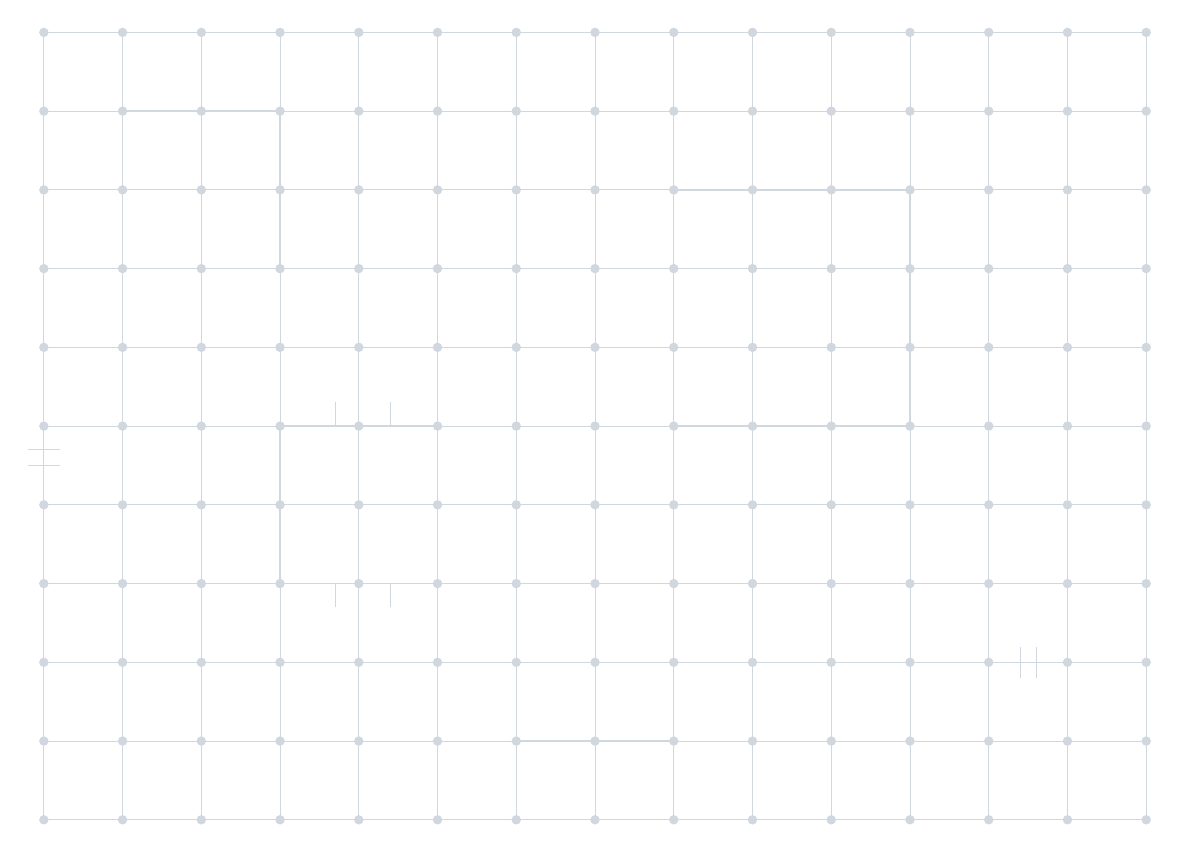
\begin{tikzpicture}[x=0.5cm,y=0.5cm]

% Very light navy color for watermark
\definecolor{circuitcolor}{RGB}{0,30,80}

\begin{scope}[circuitcolor!18!white, line width=0.3pt]

% Horizontal traces
\foreach \y in {0,2,4,6,8,10,12,14,16,18,20} {
  \draw (0,\y) -- (28,\y);
}

% Vertical traces
\foreach \x in {0,2,4,6,8,10,12,14,16,18,20,22,24,26,28} {
  \draw (\x,0) -- (\x,20);
}

% Component pads / vias at intersections (circles)
\foreach \x in {0,2,4,6,8,10,12,14,16,18,20,22,24,26,28} {
  \foreach \y in {0,2,4,6,8,10,12,14,16,18,20} {
    \fill (\x,\y) circle (0.12);
  }
}

% Short trace stubs (horizontal connectors between pads, sparse)
\foreach \y in {2,6,10,14,18} {
  \draw (2,\y) -- (4,\y);
  \draw (8,\y) -- (12,\y);
  \draw (16,\y) -- (20,\y);
  \draw (22,\y) -- (26,\y);
}

% Short trace stubs (vertical)
\foreach \x in {4,10,16,22} {
  \draw (\x,2) -- (\x,6);
  \draw (\x,10) -- (\x,14);
  \draw (\x,14) -- (\x,18);
}

% IC chip outlines (rectangles)
\draw[line width=0.5pt] (6,6) rectangle (10,10);
\draw[line width=0.5pt] (16,10) rectangle (22,16);
\draw[line width=0.5pt] (2,14) rectangle (6,18);
\draw[line width=0.5pt] (12,2) rectangle (16,6);

% Pin marks on chips
\foreach \i in {0,1,2} {
  \draw (6+\i*1.4, 6) -- (6+\i*1.4, 5.4);
  \draw (6+\i*1.4, 10) -- (6+\i*1.4, 10.6);
}
\foreach \i in {0,1} {
  \draw (6, 6+\i*2) -- (5.4, 6+\i*2);
  \draw (10, 6+\i*2) -- (10.6, 6+\i*2);
}

% Decoupling cap symbols
\draw (24,4) -- (26,4);
\draw (24.8,3.6) -- (24.8,4.4);
\draw (25.2,3.6) -- (25.2,4.4);
\draw (25.2,4) -- (26,4);

\draw (0,8) -- (0,12);
\draw (-0.4,9) -- (0.4,9);
\draw (-0.4,9.4) -- (0.4,9.4);

\end{scope}

\end{tikzpicture}
\end{document}
